% Russian language
\documentclass{article}
\usepackage[utf8]{inputenc}
\usepackage[russian]{babel}

% Math symbols
\usepackage{amssymb}
\usepackage{amsmath}

% Images inplace
\usepackage{float}
\usepackage{graphicx}

% Code blocks
\DeclareFixedFont{\ttb}{T1}{txtt}{bx}{n}{12} % for bold
\DeclareFixedFont{\ttm}{T1}{txtt}{m}{n}{12}  % for normal
\usepackage{color}
\definecolor{deepblue}{rgb}{0,0,0.5}
\definecolor{deepred}{rgb}{0.6,0,0}
\definecolor{deepgreen}{rgb}{0,0.5,0}
\usepackage{listings}
\newcommand\pythonstyle{\lstset{
language=Python,
basicstyle=\ttm,
morekeywords={self},              % Add keywords here
keywordstyle=\ttb\color{deepblue},
emph={MyClass,__init__},          % Custom highlighting
emphstyle=\ttb\color{deepred},    % Custom highlighting style
stringstyle=\color{deepgreen},
frame=tb,                         % Any extra options here
showstringspaces=false
}}
\lstnewenvironment{python}[1][]
{
\pythonstyle
\lstset{#1}
}
{}
\newcommand\pythonexternal[2][]{{
\pythonstyle
\lstinputlisting[#1]{#2}}}
\newcommand\pythoninline[1]{{\pythonstyle\lstinline!#1!}}
% Code blocks

\makeatletter
\renewcommand*\env@matrix[1][*\c@MaxMatrixCols c]{%
  \hskip -\arraycolsep
  \let\@ifnextchar\new@ifnextchar
  \array{#1}}
\makeatother

\title{Лабораторная работа №4}
\author{Ларин Егор. 4 группа 2 курс}

\begin{document}
\maketitle
\section*{Теория}
\begin{equation*}
    f(x) = e ^ {\cos x}, a = -2, b = 2, h = 0.1
\end{equation*}
\subsection*{Узлы}
\begin{equation*}
    \begin{split}
    N &= \frac{b-a}{h} + 1\\
    x_i &= a + i\cdot h, i = \overline{0, N}\\
    y_i &= f(x_i), i = \overline{0, N}
    \end{split}
\end{equation*}
\subsection*{Наилучшее приближение степени $n$}
     Линейно независимая система $\{x^0, x^1, \dots, x^n\}$:
     \begin{equation*}
         (f,g) = \sum_{k=0}^N f(x_k)g(x_k)
     \end{equation*}
\begin{equation*}
    \varphi (x) = \sum_{i=0}^n c_i \cdot x^i
\end{equation*}
Коэффициенты из решения СЛАУ
\begin{equation*}
\begin{cases}
    &c_0s_0 + c_1s_1 + \dots + c_ns_n = m_0\\
    &c_0s_1 + c_1s_2 + \dots + c_ns_{n+1} = m_1\\
    &\vdots \\
    &c_0s_{n+1} + c_1s_{n+2} + \dots + c_ns_{2n} = m_n\\
\end{cases}
\end{equation*} где
\begin{equation*}
    \begin{split}
    s_0 &= N+1\\
    s_i &= \sum_{k=0}^N x_k ^ i, \overline{1, 2n}\\
    m_0 &= \sum_{k=0}^N f(x_0)\\
    m_i &= \sum_{k=0}^N f(x_k)x_k ^ i, \overline{1, n}
    \end{split}
\end{equation*}
\subsection*{Оценка}
\begin{equation*}
     \Delta^2(f) = \sum_{i=0}^{k}(f_i - Q_n(x_i))^2 
\end{equation*}


\section*{Графики}

\begin{figure}[H]
\caption{$n=3$}
\centering
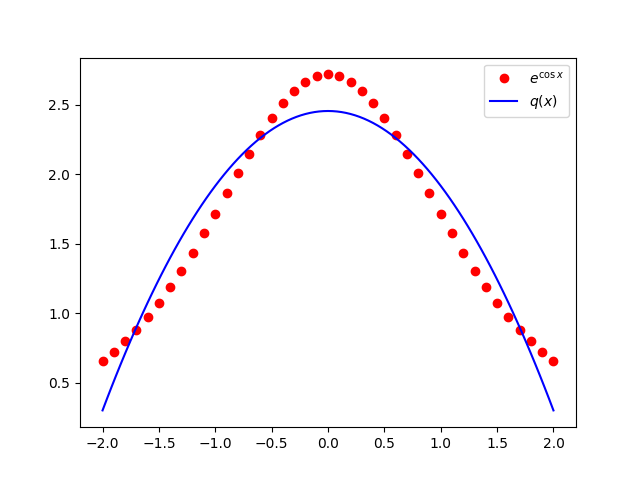
\includegraphics[width=0.9\textwidth]{3}
\end{figure}
\begin{figure}[H]
\caption{$n=6$}
\centering
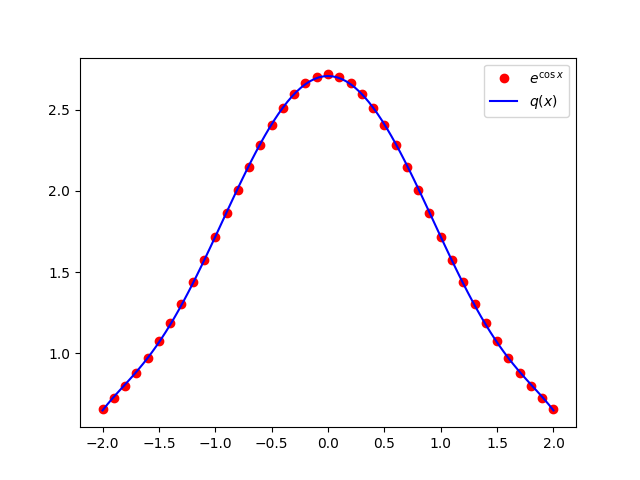
\includegraphics[width=0.9\textwidth]{6}
\end{figure}


\section*{Листинг кода}
\begin{python}
from math import cos, exp
import numpy as np
from matplotlib import pyplot as plt
h = 0.1
a = -2
b =  2
f = lambda x: exp(cos(x))
def build(n):
    k = int((b-a) / h) + 1
    xs = [a + h * i for i in range(k)]
    ys = [f(x) for x in xs]
    ss = np.array([[sum([x ** (i+j) for x in xs]) for j in range(n+1)] for i in range(n+1)])
    ms = np.array([sum([x**i * y for (x, y) in zip(xs, ys)]) for i in range(n+1)])
    cs = np.linalg.solve(ss, ms)
    q = lambda x: sum([c*(x**i) for (c,i) in zip(cs, range(n+1))])
    ds = [a + i * (b-a)/100 for i in range(101)]
    print(sum([(f(x) - q(x))**2 for x in xs]))
    plt.plot(xs, ys, "ro", ds, [q(x) for x in ds], "b")
    plt.legend(["$e^{\\cos x}$", "$q(x)$"])
    plt.show()

build(3)
build(6)
\end{python}
\section*{Результаты вычислительного эксперимента}
\begin{equation*}
   \Delta^2(f) = \sum_{i=0}^{41}(f_i - Q_3(x_i))^2 = 1.46325387355352 
\end{equation*}
\begin{equation*}
   \Delta^2(f) = \sum_{i=0}^{41}(f_i - Q_6(x_i))^2 = 0.0022915148710782995
\end{equation*}
\section*{Выводы}
Метод наименьших квадратов позволяет достаточно точно приблизить значение 
таблично заданной функции многочленом относительно невысокой степенью.
Наблюдается сходимость при увеличении степени многочлена, которая тем не менее 
на практике может и не наблюдаться из-за плохо обусловленной СЛАУ.
\end{document}